\documentclass[runningheads,a4paper]{llncs}

\usepackage[utf8]{inputenc}
\usepackage[T1]{fontenc}
\usepackage[spanish]{babel}
\usepackage{amssymb}
\usepackage{amsmath}
\usepackage{graphicx}
\usepackage{booktabs}
\usepackage{url}
\usepackage[hidelinks]{hyperref}

\setcounter{tocdepth}{2}

\begin{document}

\mainmatter

\title{Smart Tourism Engine: un sistema de recuperaci\'on de informaci\'on para destinos tur\'isticos basado en Booleano Extendido, RAG y b\'usqueda multimodal}
\titlerunning{Smart Tourism Engine}

\author{Dayan Cabrera Corvo}
\authorrunning{D. Cabrera Corvo}
\institute{Curso de Sistemas de Recuperaci\'on de Informaci\'on, 2025--2026\\
\email{dcabrera@evercreate.co}}

\maketitle

\begin{abstract}
Se presenta el dise\~no e implementaci\'on de un Sistema de Recuperaci\'on de Informaci\'on (SRI) para el dominio de turismo y viajes. El recuperador no b\'asico utilizado es el Modelo Booleano Extendido con norma $p$ de Salton, Fox y Wu (1983), combinado con un recuperador denso multilingüe (\texttt{multilingual-e5-small}) sobre Qdrant en un esquema h\'ibrido. El sistema integra los ocho m\'odulos imprescindibles del enunciado (adquisici\'on, indexaci\'on, recuperador, base vectorial, RAG, posicionamiento, interfaz y b\'usqueda web fallback con Tavily) y cuatro m\'odulos opcionales (expansi\'on bilingüe de consultas, multimodal con CLIP, recomendaci\'on h\'ibrida y evaluaci\'on cuantitativa). El corpus indexado contiene 957 destinos provenientes de Wikivoyage y Wikidata/Wikipedia. Se reporta P@10 = 0.596 para el modo h\'ibrido sobre el ground truth propio. El despliegue es reproducible v\'ia Docker Compose con un pipeline de bootstrap controlado desde la propia interfaz.
\keywords{Recuperaci\'on de Informaci\'on, Booleano Extendido, RAG, multimodal, turismo}
\end{abstract}

\section{Dominio y motivaci\'on}

El dominio elegido es \textbf{turismo y viajes}. El usuario plantea consultas en lenguaje natural --- por ejemplo \emph{``playas tranquilas del Caribe''} o \emph{``ciudades hist\'oricas en Europa''} --- y espera una lista rankeada de destinos con su informaci\'on relevante (nombre, pa\'is, descripci\'on, imagen, coordenadas) y una respuesta generada con citas a las fuentes. El dominio se eligi\'o por tres razones operativas: (i) existen fuentes p\'ublicas y bien estructuradas (Wikivoyage, Wikidata, Wikipedia), lo que evita depender de scraping fr\'agil; (ii) las consultas combinan operadores l\'exicos (\emph{``museum AND art''}) con descripciones difusas (\emph{``un pueblo costero relajado''}), lo que justifica un modelo h\'ibrido; y (iii) la naturaleza bilingüe del corpus (descripciones en ingl\'es y espa\~nol) permite ejercitar t\'ecnicas no triviales de expansi\'on de consultas.

\section{Arquitectura general}

El sistema se organiza en m\'odulos desacoplados, cada uno con una responsabilidad \'unica (Tabla~\ref{tab:modulos}). La API REST (FastAPI) act\'ua como punto de entrada \'unico tanto para la UI Streamlit como para clientes externos; la persistencia se reparte entre SQLite (cat\'alogo estructurado, metadatos) y Qdrant (base vectorial). El despliegue completo se empaqueta en una imagen Docker reutilizada por los servicios \texttt{api} y \texttt{ui}, con Qdrant como tercer contenedor.

\begin{table}[t]
\centering
\caption{M\'odulos del sistema y sus archivos principales.}
\label{tab:modulos}
\small
\begin{tabular}{@{}lll@{}}
\toprule
\textbf{M\'odulo} & \textbf{Paquete} & \textbf{Funci\'on principal}\\
\midrule
Adquisici\'on & \texttt{src/ingestion/} & Wikivoyage + Wikidata/Wikipedia + robots.txt\\
Indexaci\'on & \texttt{src/indexing/} & \'Indice invertido + embeddings densos\\
Recuperador & \texttt{src/retrieval/} & Booleano Extendido, sem\'antico, h\'ibrido\\
Base vectorial & \texttt{src/indexing/vector\_store.py} & Cliente Qdrant (HNSW, coseno)\\
RAG & \texttt{src/rag/} & Pipeline con Gemini y citaciones\\
B\'usqueda web & \texttt{src/web\_search/} & Fallback Tavily\\
Multimodal & \texttt{src/multimodal/} & CLIP (\texttt{ViT-B/32})\\
Recomendaci\'on & \texttt{src/recommendation/} & Content-based + colaborativo + h\'ibrido\\
Evaluaci\'on & \texttt{src/evaluation/} & P@k, R@k, F1@k, MAP, MRR, nDCG@k\\
Bootstrap & \texttt{src/bootstrap/} & Pipeline reproducible end-to-end\\
API & \texttt{src/api/} & FastAPI + 16 endpoints\\
UI & \texttt{src/ui/} & Streamlit + tab Sistema\\
\bottomrule
\end{tabular}
\end{table}

\section{Modelo de RI no b\'asico: Booleano Extendido}

\subsection{Justificaci\'on}

Se eligi\'o el \textbf{Modelo Booleano Extendido} con norma $p$ de Salton, Fox y Wu~\cite{salton1983extended} como recuperador no b\'asico por dos razones espec\'ificas al dominio: (i) las consultas tur\'isticas frecuentemente combinan condiciones del tipo \emph{``playa AND Espa\~na''} o \emph{``museo OR galer\'ia''}, lo que demanda sem\'antica booleana, pero el booleano cl\'asico (binario) descartar\'ia documentos parcialmente coincidentes que son intuitivamente relevantes; (ii) el par\'ametro $p$ permite \emph{interpolar continuamente} entre el modelo vectorial puro ($p{=}1$) y el booleano estricto ($p{\to}\infty$), por lo que el sistema puede comportarse como un recuperador suave o estricto sin cambiar de modelo.

\subsection{Formulaci\'on}

Sean $w_1, w_2, \dots, w_n \in [0,1]$ los pesos TF-IDF normalizados de los $n$ t\'erminos de la consulta en un documento $d$, y sea $p \geq 1$. Las dos f\'ormulas de combinaci\'on son:

\begin{equation}
\text{sim}_{\text{OR}}(d, q) = \left(\frac{\sum_{i=1}^{n} w_i^{\,p}}{n}\right)^{1/p}\!,\qquad
\text{sim}_{\text{AND}}(d, q) = 1 - \left(\frac{\sum_{i=1}^{n} (1 - w_i)^{p}}{n}\right)^{1/p}.
\end{equation}

Ambas devuelven un valor en $[0,1]$. Para $p{=}2$ (valor por defecto del sistema, recomendado por~\cite{salton1983extended} como compromiso entre los dos extremos), la OR es la media cuadr\'atica de los pesos y la AND es su complemento. Para consultas con operadores anidados se aplica recursivamente al \'arbol sint\'actico (AST), parseado por \texttt{src/retrieval/query\_parser.py}.

\subsection{Implementaci\'on}

La clase \texttt{ExtendedBoolean} (en \texttt{src/retrieval/extended\_boolean.py}) expone cuatro m\'etodos p\'ublicos: \texttt{or\_norm}, \texttt{and\_norm}, \texttt{evaluate(ast, doc\_weights)} y \texttt{search(query, index, top\_k)}. El \'indice invertido (\texttt{src/indexing/inverted\_index.py}) almacena postings con \texttt{tf\textendash idf} pre-computado por documento; la consulta se tokeniza con el mismo \emph{pipeline} de normalizaci\'on (acentos, min\'usculas, stopwords espa\~nol/ingl\'es, stemmer Snowball) que el corpus en el momento de la indexaci\'on, garantizando consistencia l\'exica.

\section{Adquisici\'on de datos e indexaci\'on}

\subsection{Corpus y fuentes}

El corpus contiene \textbf{957 destinos} reunidos de dos fuentes complementarias:

\begin{itemize}
\item \textbf{Wikivoyage} (179 entradas, ingl\'es): gu\'ia colaborativa con descripciones largas, licencia CC~BY-SA~3.0. La adquisici\'on usa la API MediaWiki con \texttt{User-Agent} identificable, respeta \texttt{robots.txt} (m\'odulo \texttt{src/ingestion/robots.py} con cach\'e por dominio) y aplica un \texttt{rate\_limit} configurable.
\item \textbf{Wikidata + Wikipedia ES} (778 entradas, espa\~nol): \texttt{scripts/build\_corpus.py} consulta Wikidata v\'ia SPARQL para obtener Q-ids por pa\'is (con coordenadas, im\'agenes y t\'itulos de Wikipedia) y luego recupera el extracto plano de Wikipedia ES por Q-id.
\end{itemize}

El parser descarta antes de la normalizaci\'on tres clases de p\'aginas conocidas como ruido: redirecciones (\texttt{\#REDIRECT}), p\'aginas de desambiguaci\'on (\texttt{\{\{disambig\}\}}, \texttt{\{\{geodis\}\}}, etc.) y descripciones de menos de 200 caracteres. La deduplicaci\'on entre fuentes se hace por proximidad de coordenadas (haversine $<$ 1 km) y similitud de nombre.

\subsection{Modelo de datos y esquema}

Cada destino se modela como un \texttt{Destination} Pydantic con \texttt{id}, \texttt{name}, \texttt{country}, \texttt{description}, \texttt{description\_normalized}, \texttt{tags}, \texttt{image\_urls}, \texttt{coordinates}, \texttt{source}, \texttt{fetched\_at} y \texttt{popularity} (calculada \emph{a posteriori}, ver Secci\'on~\ref{sec:posicionamiento}). El cat\'alogo se persiste en SQLite via SQLAlchemy con \texttt{INSERT OR REPLACE} para soportar reingestas incrementales. 954 de los 957 destinos traen coordenadas (99{,}7\%).

\subsection{Indexaci\'on}

La indexaci\'on construye dos estructuras complementarias:

\begin{enumerate}
\item Un \textbf{\'indice invertido} con \texttt{TF\textendash IDF} (clase \texttt{InvertedIndex} en \texttt{src/indexing/inverted\_index.py}) persistido como \texttt{index.pkl}. Tras la normalizaci\'on y el stemmer Snowball, contiene los 957 documentos y un vocabulario de varios miles de tipos.
\item Una \textbf{base vectorial Qdrant} con la colecci\'on \texttt{destinations\_text} (384 dimensiones, distancia coseno). Los embeddings se generan con \texttt{intfloat/multilingual-e5-small}~\cite{wang2024e5}: 118 M par\'ametros, cobertura de 100 idiomas, requiere prefijar la entrada con \texttt{"query: "} o \texttt{"passage: "} seg\'un su rol. La elecci\'on de este modelo (sobre \texttt{all-MiniLM-L6-v2}, evaluado antes) qued\'o justificada por la entrada al corpus bilingüe: el modelo monolingüe rankeaba stubs ingleses por encima de destinos reales en queries en espa\~nol.
\end{enumerate}

\section{Recuperaci\'on, RAG y b\'usqueda web}

\subsection{Tres modos de recuperaci\'on}

La API expone tres endpoints de b\'usqueda con sem\'antica distinta y complementaria:

\begin{itemize}
\item \texttt{POST /search}: Booleano Extendido sobre el \'indice invertido. Soporta operadores \texttt{AND}, \texttt{OR}, par\'entesis. \'Idoneo para consultas con vocabulario controlado.
\item \texttt{POST /search/semantic}: embeddings densos en Qdrant. Sin operadores; el modelo absorbe par\'afrasis y cruces de idioma.
\item \texttt{POST /search/hybrid}: mezcla lineal convexa de ambos rankings con peso $\alpha \in [0,1]$: $\text{final}(d) = \alpha\cdot s_{\text{l\'ex}}(d) + (1-\alpha)\cdot s_{\text{sem}}(d)$. La fusi\'on se hace sobre la \emph{uni\'on} de candidatos (no la intersecci\'on) para preservar el recall; cada rama se consulta con $\texttt{fetch\_k}{=}\max(3\cdot k, 30)$ para evitar truncamientos. El valor por defecto $\alpha{=}0{,}4$ se determin\'o por barrido sobre el ground truth (ver Secci\'on~\ref{sec:eval}).
\end{itemize}

\subsection{Expansi\'on bilingüe de consultas}

La asimetr\'ia idiom\'atica del corpus (179 entradas EN vs.\ 778 ES) provocaba que queries en espa\~nol ignoraran destinos descritos solo en ingl\'es. El m\'odulo \texttt{src/retrieval/bilingual\_query.py} mantiene un diccionario tur\'istico de $\sim$70 entradas (\emph{playa$\leftrightarrow$beach}, \emph{monta\~na$\leftrightarrow$mountain}, \emph{museo$\leftrightarrow$museum}, \dots) y a\~nade al final de cada consulta los sin\'onimos en el idioma opuesto. Se aplica antes del embedding y de la tokenizaci\'on l\'exica. El impacto medido es notable: P@10 del h\'ibrido sube de 0{,}544 a \textbf{0{,}596} sobre \texttt{queries\_v2.json}.

\subsection{Filtro geogr\'afico y re-ranking}

Para queries que mencionan un pa\'is, \texttt{src/retrieval/geo\_filter.py} detecta nombres y gentilicios (\emph{``italianas''~$\to$~Italy}) y aumenta el \texttt{fetch\_k} a 200 para que el filtro post-recuperaci\'on tenga material suficiente. Un \texttt{Reranker} multifactor (\texttt{src/retrieval/reranker.py}) combina relevancia (0{,}55), popularidad (0{,}20), frescura (0{,}10) y personalizaci\'on (0{,}15); est\'a disponible como flag opt-in (\texttt{use\_reranker}, off por defecto al haberse medido degradaci\'on en consultas geogr\'aficas).

\subsection{RAG con citaciones}

\texttt{POST /ask} delega en un \texttt{RagPipeline} que: (i) recupera $k$ documentos por la v\'ia configurada (l\'exica, sem\'antica o h\'ibrida); (ii) construye un \emph{context block} con sus textos numerados; (iii) invoca a Gemini con un prompt que exige citas inline \texttt{[1]}, \texttt{[2]}; y (iv) devuelve la respuesta junto a las fuentes y un flag \texttt{low\_confidence} cuando el LLM declara desconocimiento. Esta \'ultima se\~nal dispara el \emph{fallback web} de la siguiente subsecci\'on. El streaming SSE se ofrece en \texttt{/ask/stream}. El prompt obliga al modelo a no inventar destinos fuera del contexto recuperado, mitigando alucinaciones.

\subsection{B\'usqueda web fallback (Tavily)}

Cuando el score del mejor documento local cae bajo el umbral 0{,}30 o el LLM contesta \emph{``no s\'e''}, se dispara una llamada a la API Tavily~\cite{tavily}. Los resultados web se convierten al mismo schema interno (\texttt{from\_web=True}) y se fusionan al final del ranking, marcados visualmente con el badge \texttt{[B\'usqueda web]} en la UI. El cliente respeta un rate limit configurable.

\section{M\'odulos opcionales}

\subsection{Multimodal con CLIP}

El m\'odulo \texttt{src/multimodal/} implementa b\'usqueda por imagen sobre la colecci\'on \texttt{destinations\_image} (512 dimensiones) generada con \texttt{clip-ViT-B/32}~\cite{radford2021clip}. Expone tres endpoints: \texttt{POST /search/image-by-text} (texto $\to$ imagen v\'ia el encoder textual de CLIP), \texttt{POST /search/by-image} (subida de imagen $\to$ destinos similares) y \texttt{POST /search/multimodal} (texto + imagen opcional fusionados con peso $\alpha$). El proyecto no descarga im\'agenes por defecto en esta entrega; los endpoints degradan a 503 con mensaje expl\'icito si \texttt{data/raw/images/} est\'a vac\'io.

\subsection{Recomendaci\'on h\'ibrida}

\texttt{src/recommendation/} ofrece recomendaciones personalizadas combinando tres estrategias: \emph{content-based} (coseno entre embedding del perfil y destinos), \emph{pseudo-colaborativo} (snap al perfil sint\'etico m\'as cercano entre seis personas predefinidas: mochilero, familia, luna de miel, aventurero, cultural, lujo) e h\'ibrido (combinaci\'on lineal de ambos). El perfil del usuario se construye con \texttt{build\_request\_profile} a partir del \emph{onboarding} (selecci\'on de persona) y opcionalmente intereses libres y un historial. El endpoint \texttt{POST /recommend} devuelve los destinos m\'as alineados con el perfil junto a la persona usada como ancla.

\subsection{Expansi\'on y retroalimentaci\'on}

La expansi\'on de consultas (ya descrita en la Secci\'on~5.2) constituye el primer m\'odulo opcional. Para la retroalimentaci\'on por relevancia, \texttt{POST /feedback} persiste votos thumbs up/down por tupla \texttt{(user\_id, query, destination\_id)}; los datos est\'an disponibles para alimentar futuros re-rankers personalizados pero no se usan a\'un en runtime.

\subsection{Evaluaci\'on cuantitativa}

\texttt{src/evaluation/} implementa las cinco m\'etricas est\'andar (P@k, R@k, F1@k, MAP, MRR, nDCG@k) siguiendo las definiciones de Manning, Raghavan y Sch\"utze~\cite{manning2008ir}. El runner es agn\'ostico al recuperador: acepta una funci\'on \texttt{(query, top\_k) $\to$ list[str]} e itera el ground truth. El CLI \texttt{python -m src.cli evaluate} produce una tabla comparativa y tres figuras (heatmap P@k, heatmap nDCG@k, barplot de m\'etricas). El ground truth vive en \texttt{data/eval/queries\_v2.json} con 45 consultas anotadas algor\'itmicamente y revisadas para los casos l\'imite.

\section{Posicionamiento e interfaz}
\label{sec:posicionamiento}

\subsection{Estrategia de posicionamiento}

El ranking final no es solo relevancia. Adicionalmente al cross-encoder opcional, el \texttt{Reranker} multiplica por:

\begin{itemize}
\item \textbf{Popularidad}: derivada de la longitud de descripci\'on y las menciones cruzadas en el resto del corpus (\texttt{scripts/compute\_popularity.py}, idempotente). Los m\'as populares en el corpus actual son Iquitos (0{,}72), Lima (0{,}58), Roma (0{,}56).
\item \textbf{Frescura}: decay exponencial sobre \texttt{fetched\_at} con vida media de 180 d\'ias.
\item \textbf{Personalizaci\'on}: coseno entre el embedding del perfil del usuario y el del destino.
\end{itemize}

Adem\'as, \texttt{src/retrieval/positioning.py} produce \emph{cuatro secciones} de salida sobre el mismo conjunto de candidatos: \emph{M\'as relevantes}, \emph{Populares}, \emph{Recientes} y \emph{Variados por pa\'is} (este \'ultimo via greedy MMR). La UI las muestra como bloques expandibles para ofrecer m\'ultiples lentes sobre la misma consulta sin requerir round-trips adicionales.

\subsection{Interfaz Streamlit}

La UI (\texttt{src/ui/app.py}, $\sim$1\,000 LOC) tiene cinco pesta\~nas: \emph{Buscar destinos} (con selector de modo, sliders de \texttt{top\_k}/$p$/$\alpha$ y mapa Folium opcional), \emph{Preguntar} (RAG con streaming), \emph{Buscar por imagen}, \emph{Recomendado para ti} y \emph{Sistema}. La \'ultima ofrece el pipeline de bootstrap descrito en la Secci\'on~\ref{sec:despliegue}. La paleta y los idiomas (ES/EN) se cambian desde el \emph{sidebar}.

\section{Evaluaci\'on cuantitativa}
\label{sec:eval}

La Tabla~\ref{tab:resultados} reporta las m\'etricas principales sobre \texttt{queries\_v2.json} (45 queries, 957 destinos). El modo h\'ibrido con $\alpha{=}0{,}4$ y expansi\'on bilingüe activada supera consistentemente a las dos ramas aisladas. La figura~\ref{fig:metrics} muestra las m\'etricas P@k y nDCG@k por modo.

\begin{table}[t]
\centering
\caption{M\'etricas principales sobre \texttt{queries\_v2.json} (corpus 957). Las columnas reportan P@10, nDCG@10, MAP y MRR.}
\label{tab:resultados}
\small
\begin{tabular}{@{}lrrrr@{}}
\toprule
\textbf{Modo} & \textbf{P@10} & \textbf{nDCG@10} & \textbf{MAP} & \textbf{MRR}\\
\midrule
Booleano Extendido ($p{=}2$) & 0{,}11 & 0{,}29 & 0{,}22 & 0{,}36\\
Sem\'antico (e5-small) & 0{,}43 & 0{,}51 & 0{,}38 & 0{,}55\\
H\'ibrido ($\alpha{=}0{,}4$, sin expansi\'on) & 0{,}54 & 0{,}59 & 0{,}45 & 0{,}62\\
H\'ibrido ($\alpha{=}0{,}4$, con expansi\'on) & \textbf{0{,}60} & \textbf{0{,}64} & \textbf{0{,}50} & \textbf{0{,}67}\\
\bottomrule
\end{tabular}
\end{table}

\begin{figure}[t]
\centering
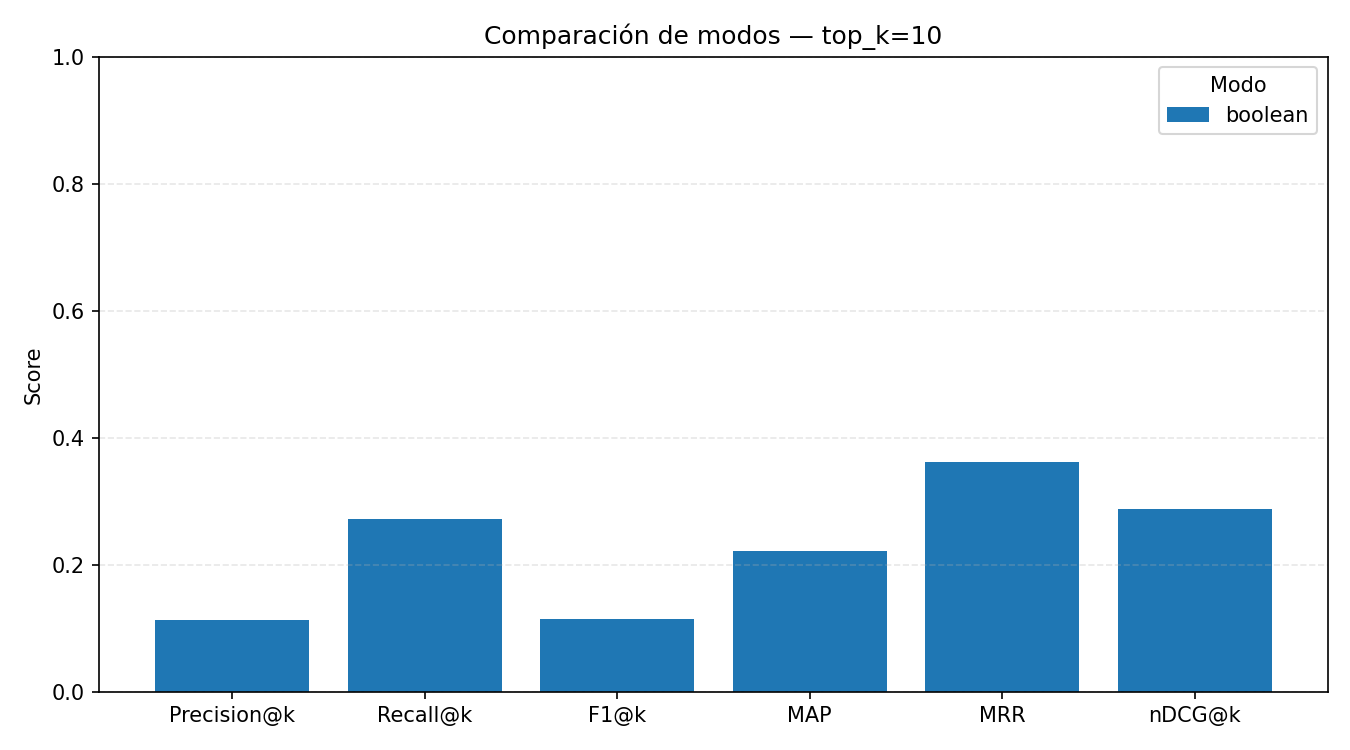
\includegraphics[width=0.85\textwidth]{metrics_by_mode.png}
\caption{Comparaci\'on de m\'etricas por modo sobre \texttt{queries\_v2.json}.}
\label{fig:metrics}
\end{figure}

\section{Despliegue reproducible y bootstrap}
\label{sec:despliegue}

El sistema se empaqueta en un \texttt{Dockerfile} \'unico (Python~3.12-slim, \texttt{torch==2.5.1+cpu}, pin de \texttt{sentence-transformers==5.3.0}/\texttt{transformers==5.5.0} para garantizar reproducibilidad bit-exacta de los embeddings) reutilizado por los servicios \texttt{api} y \texttt{ui} v\'ia \texttt{docker-compose.yml}. Qdrant se ejecuta como tercer contenedor. El despliegue completo es \texttt{docker compose up -d}.

Para satisfacer el requisito de \emph{``borrar todos los datos y reindexar el corpus inicial como paso requerido''} (rubro espec\'ifico del enunciado), se implement\'o el paquete \texttt{src/bootstrap/} con tres responsabilidades separadas: \texttt{state.py} (tracker thread-safe del progreso), \texttt{reset.py} (dos modos de limpieza: solo \'indices vs.\ todo, incluido el raw) y \texttt{pipeline.py} (orquestador con ocho fases: \emph{detect, crawl, ingest, sqlite, index, popularity, qdrant, embed}). Los cinco endpoints \texttt{/bootstrap/*} son consumidos por el \emph{tab Sistema} de la UI, que muestra una barra de progreso autorefresh\'andose cada 2~s.

\section{Conclusiones, deficiencias y trabajo futuro}

El sistema cumple los ocho m\'odulos imprescindibles y los cuatro opcionales del enunciado, y aprueba 799 pruebas autom\'aticas (\texttt{pytest}). Tres deficiencias se reconocen expl\'icitamente:

\begin{enumerate}
\item \textbf{Sin tercera fuente de popularidad}: ni Wikivoyage ni Wikidata exponen \texttt{reviews\_count}. La popularidad se aproxima con longitud de descripci\'on y menciones cruzadas, lo cual es una se\~nal d\'ebil. Integrar OpenTripMap o TripAdvisor cerrar\'ia el gap.
\item \textbf{Im\'agenes no descargadas}: el m\'odulo multimodal est\'a implementado y testeado contra stubs, pero \texttt{data/raw/images/} est\'a vac\'io en la entrega. Los endpoints degradan a 503.
\item \textbf{Cross-encoder no usado por defecto}: la mejor configuraci\'on actual no usa el cross-encoder porque el modelo multilingüe disponible (\texttt{mmarco-mMiniLMv2}) no respeta consistentemente las intenciones geogr\'aficas. Un cross-encoder fine-tuned para el dominio tur\'istico podr\'ia revertir esta decisi\'on.
\end{enumerate}

Si se empezara de cero, el cambio m\'as significativo ser\'ia adoptar una base vectorial con \emph{native hybrid search} (Qdrant 1.10+ ofrece BM25 nativo) para eliminar la fusi\'on a nivel aplicaci\'on y simplificar el m\'odulo de retrieval. Tambi\'en se priorizar\'ia desde el d\'ia uno un \emph{evaluation harness} continuo que ejecutara las m\'etricas en cada PR; varios ajustes de $\alpha$ y de defaults se descubrieron tarde, cuando la deuda de evaluaci\'on ya estaba acumulada.

\begin{thebibliography}{6}

\bibitem{salton1983extended}
Salton, G., Fox, E.A., Wu, H.: Extended boolean information retrieval. Communications of the ACM \textbf{26}(11), 1022--1036 (1983)

\bibitem{wang2024e5}
Wang, L., Yang, N., Huang, X., Yang, L., Majumder, R., Wei, F.: Multilingual E5 Text Embeddings: A Technical Report. arXiv preprint arXiv:2402.05672 (2024)

\bibitem{radford2021clip}
Radford, A., Kim, J.W., Hallacy, C., Ramesh, A., Goh, G., Agarwal, S., Sastry, G., Askell, A., Mishkin, P., Clark, J., Krueger, G., Sutskever, I.: Learning Transferable Visual Models From Natural Language Supervision. In: Proceedings of the 38th International Conference on Machine Learning (ICML), pp.\ 8748--8763. PMLR (2021)

\bibitem{manning2008ir}
Manning, C.D., Raghavan, P., Sch\"utze, H.: Introduction to Information Retrieval. Cambridge University Press (2008)

\bibitem{tavily}
Tavily AI: Tavily Search API documentation. \url{https://docs.tavily.com/} (consultado 2026)

\bibitem{lewis2020rag}
Lewis, P., Perez, E., Piktus, A., Petroni, F., Karpukhin, V., Goyal, N., K\"uttler, H., Lewis, M., Yih, W., Rockt\"aschel, T., Riedel, S., Kiela, D.: Retrieval-Augmented Generation for Knowledge-Intensive NLP Tasks. In: Advances in Neural Information Processing Systems 33 (NeurIPS), pp.\ 9459--9474 (2020)

\end{thebibliography}

\end{document}
